\chapter{Optoelektronické součástky používané při laser game}

\section{Optické vysílače}
Optické vysílače obdobně jako vysílače rádiové slouží k vysílání elektromagnetických vln. Od rádiových vysílačů  se odlišují tím, že využívají jinou část elektromagnetického spektra $\lambda \in \langle 10~\jedn{nm}~;~1~\jedn{mm}  \rangle$, tedy od infračerveného záření, přes viditelné světlo až po záření ultra fialové. Vysílače můžeme rozdělit do dvou skupin a to vysílače založené na \zkratka{LED} a na laseru.

\subsubsection{LED}
Luminiscenční diody jsou polovodičové součástky s jedním PN přechodem. Na rozdíl od klasických diod nemají \zkratka{LED} obě vrstvy PN přechodu stejně dotované. Polovodič N je mnohem více dotován, navíc má mnohem větší objem než polovodič P. Díky tomu, pokud diodou prochází proud, převažuje přesun nosičů z oblasti N do oblasti P, kde rekombinují a uvolněná energie je přeměněna na světelné záření a tepelnou energii. Vrstva P je tenká, aby nedocházelo k velkým ztrátám při šíření světla z polovodiče do okolního prostředí. Vlnová délka vyzařovaného světla je dána použitým základním materiálem. Pokud známe vlnovou délku, je možné spočítat potřebou energii, kterou je třeba elektronům udělit, aby \zkratka{LED} svítila.

$$ E = hf = \dfrac{hc}{\lambda} $$

\begin{figure}[H]
    \begin{center}
        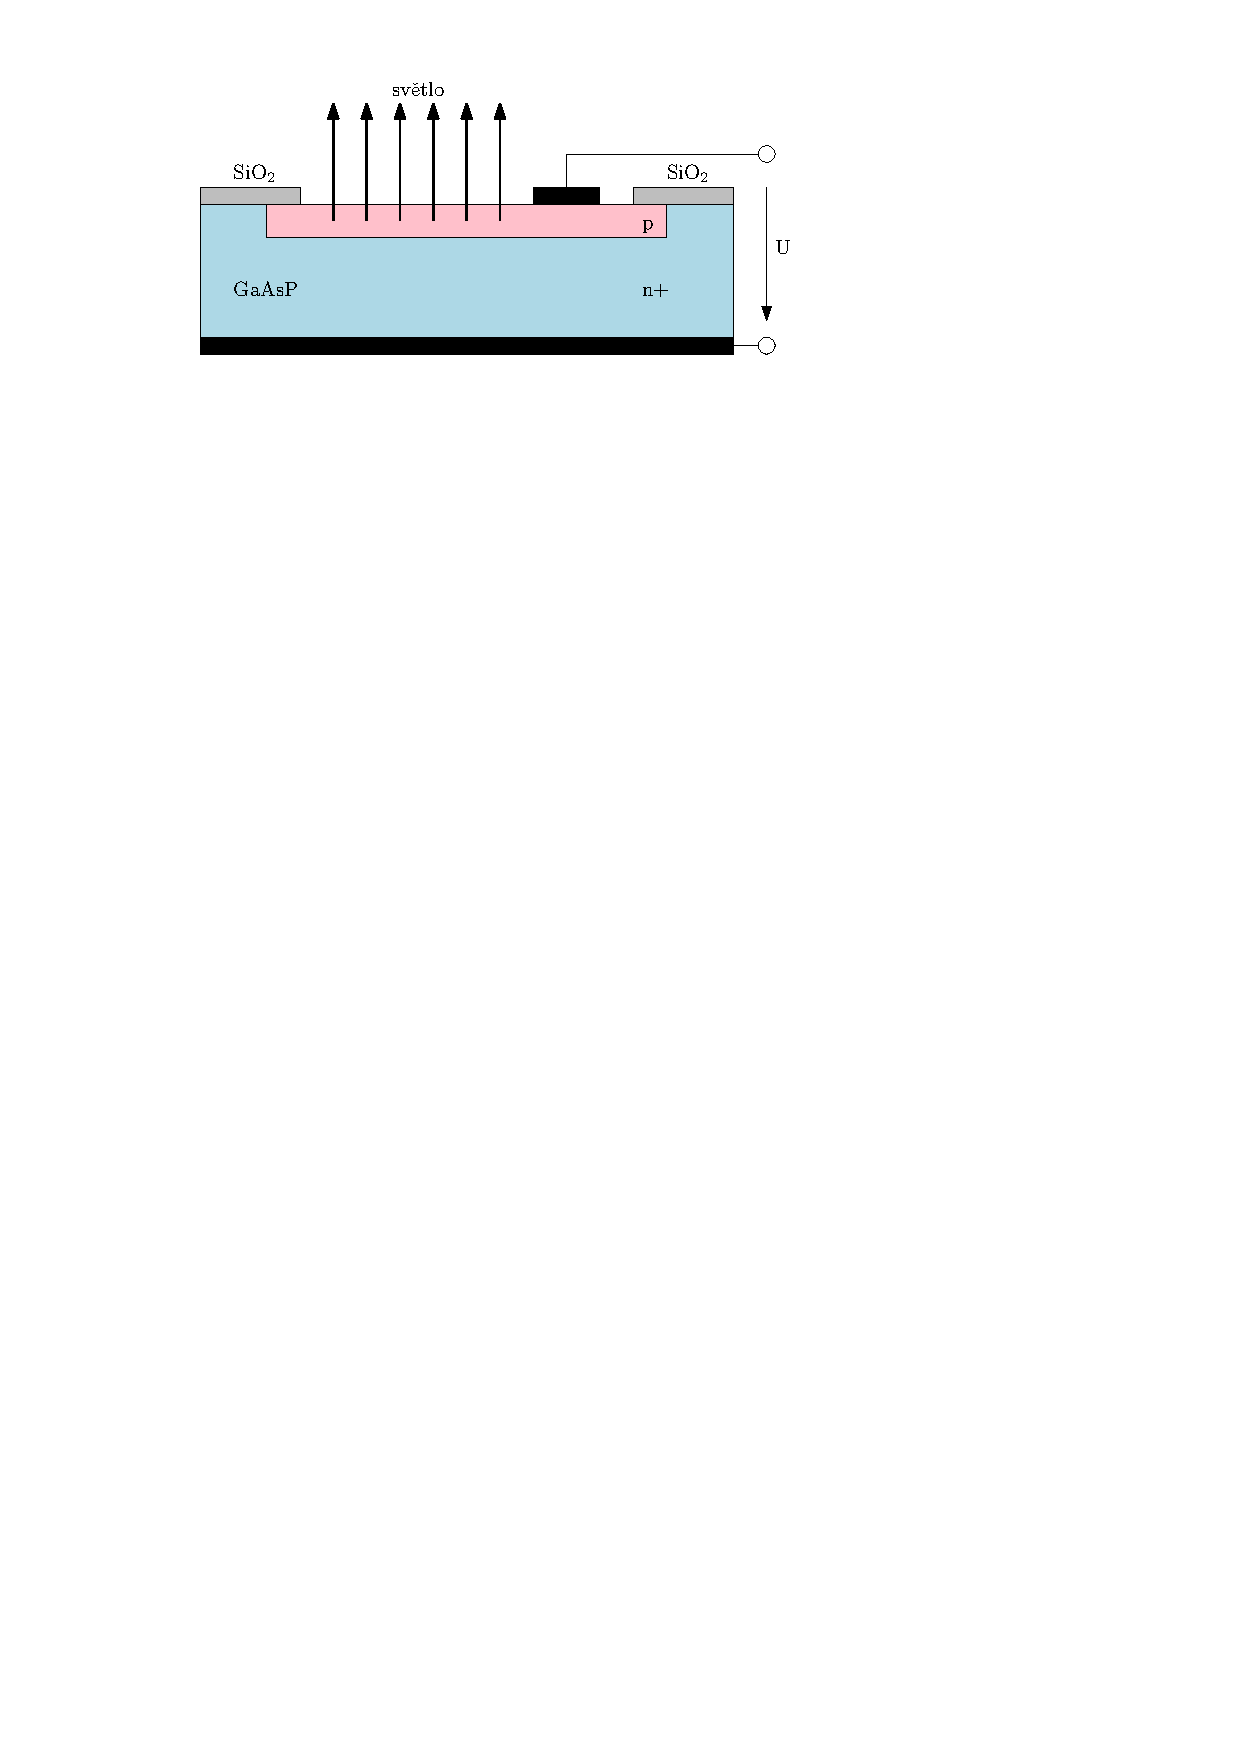
\includegraphics[scale=1]{img/led}
    \end{center}
    \caption{Technologické provedení LED pro viditelné světlo}
\end{figure}

\begin{figure}[H]
    \begin{center}
        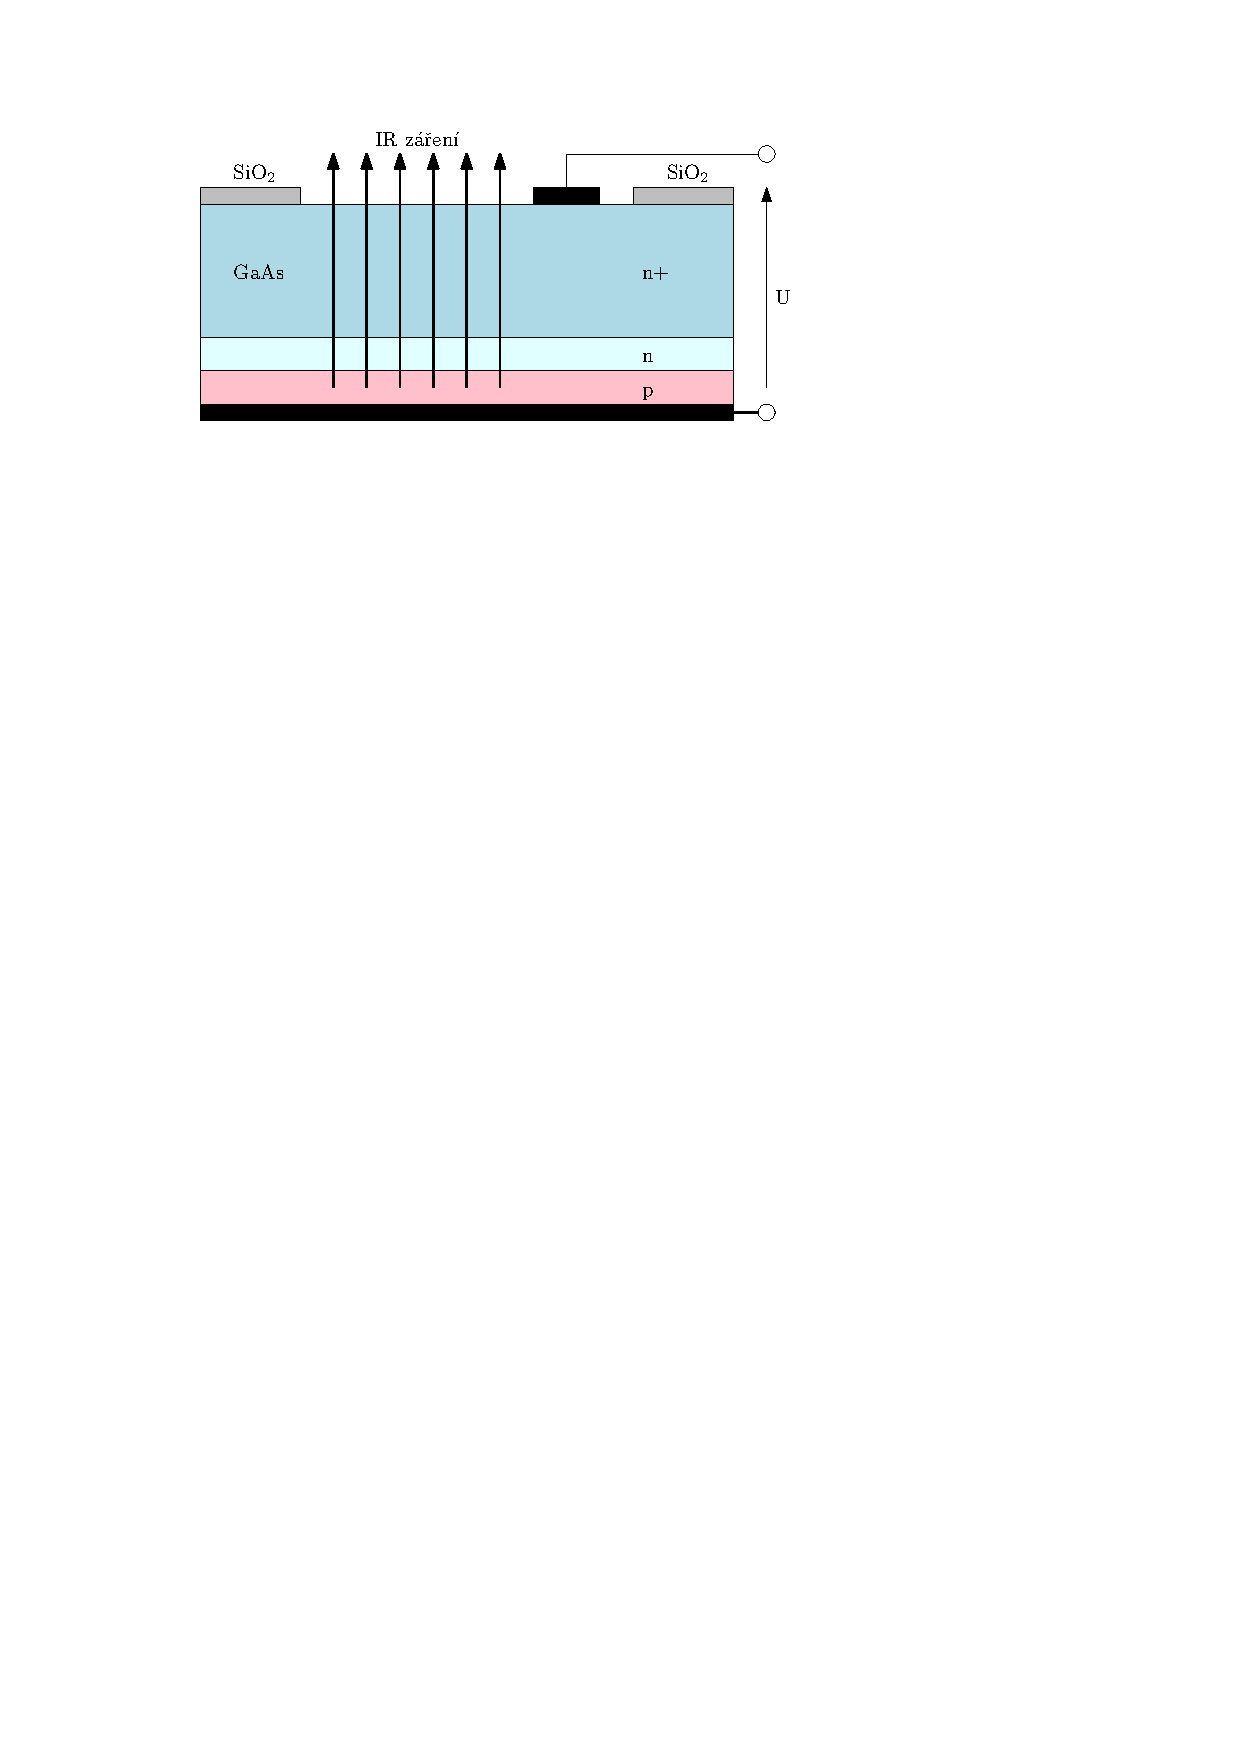
\includegraphics[scale=1]{img/ir-led}
    \end{center}
    \caption{Technologické provedení IR LED}
\end{figure}

\zkratka{IR} \zkratka{LED} jsou konstrukčně řešeny jinak. Využívá se toho, že \zkratka{IR} záření není polovodičem tlumeno tolik jako viditelné světlo. Díky tomu mohla být oblast vzniku záření umístěna do spodní části substrátu. To má velkou výhodu, protože se může snáze odvádět teplo vznikající při rekombinaci. Díky tomu mohou \zkratka{IR} \zkratka{LED} vyzařovat mnohem větší výkon než diody vyzařující viditelné světlo. Proto nalézají uplatnění jako optické vysílače, zejména na delší vzdálenosti. Základním materiálem pro výrobu \zkratka{IR} \zkratka{LED} je galiumarsenit. Vyráběné diody dosahují vlnových délek $\lambda \in \langle 830~\jedn{nm}~;~1040~\jedn{nm} \rangle$.

\subsubsection{Laserové diody}
Laserová dioda je polovodičová součástka, která při malém proudu v propustném směru se chová jako klasická luminiscenční dioda. Proud způsobí spontánní emisi, což znamená, že k emisi dochází náhodně v libovolný čas, čímž dioda vyzařuje světelné záření. Při zvýšení proudu diodou přechází dioda do laserového režimu. V tomto režimu je vyzařované světlo koherentní, tedy má konstantní frekvenci a fázi. To nastane díky optické rezonanci v polovodičovém krystalu a následné vynucené emisi.

\begin{figure}[H]
    \begin{center}
        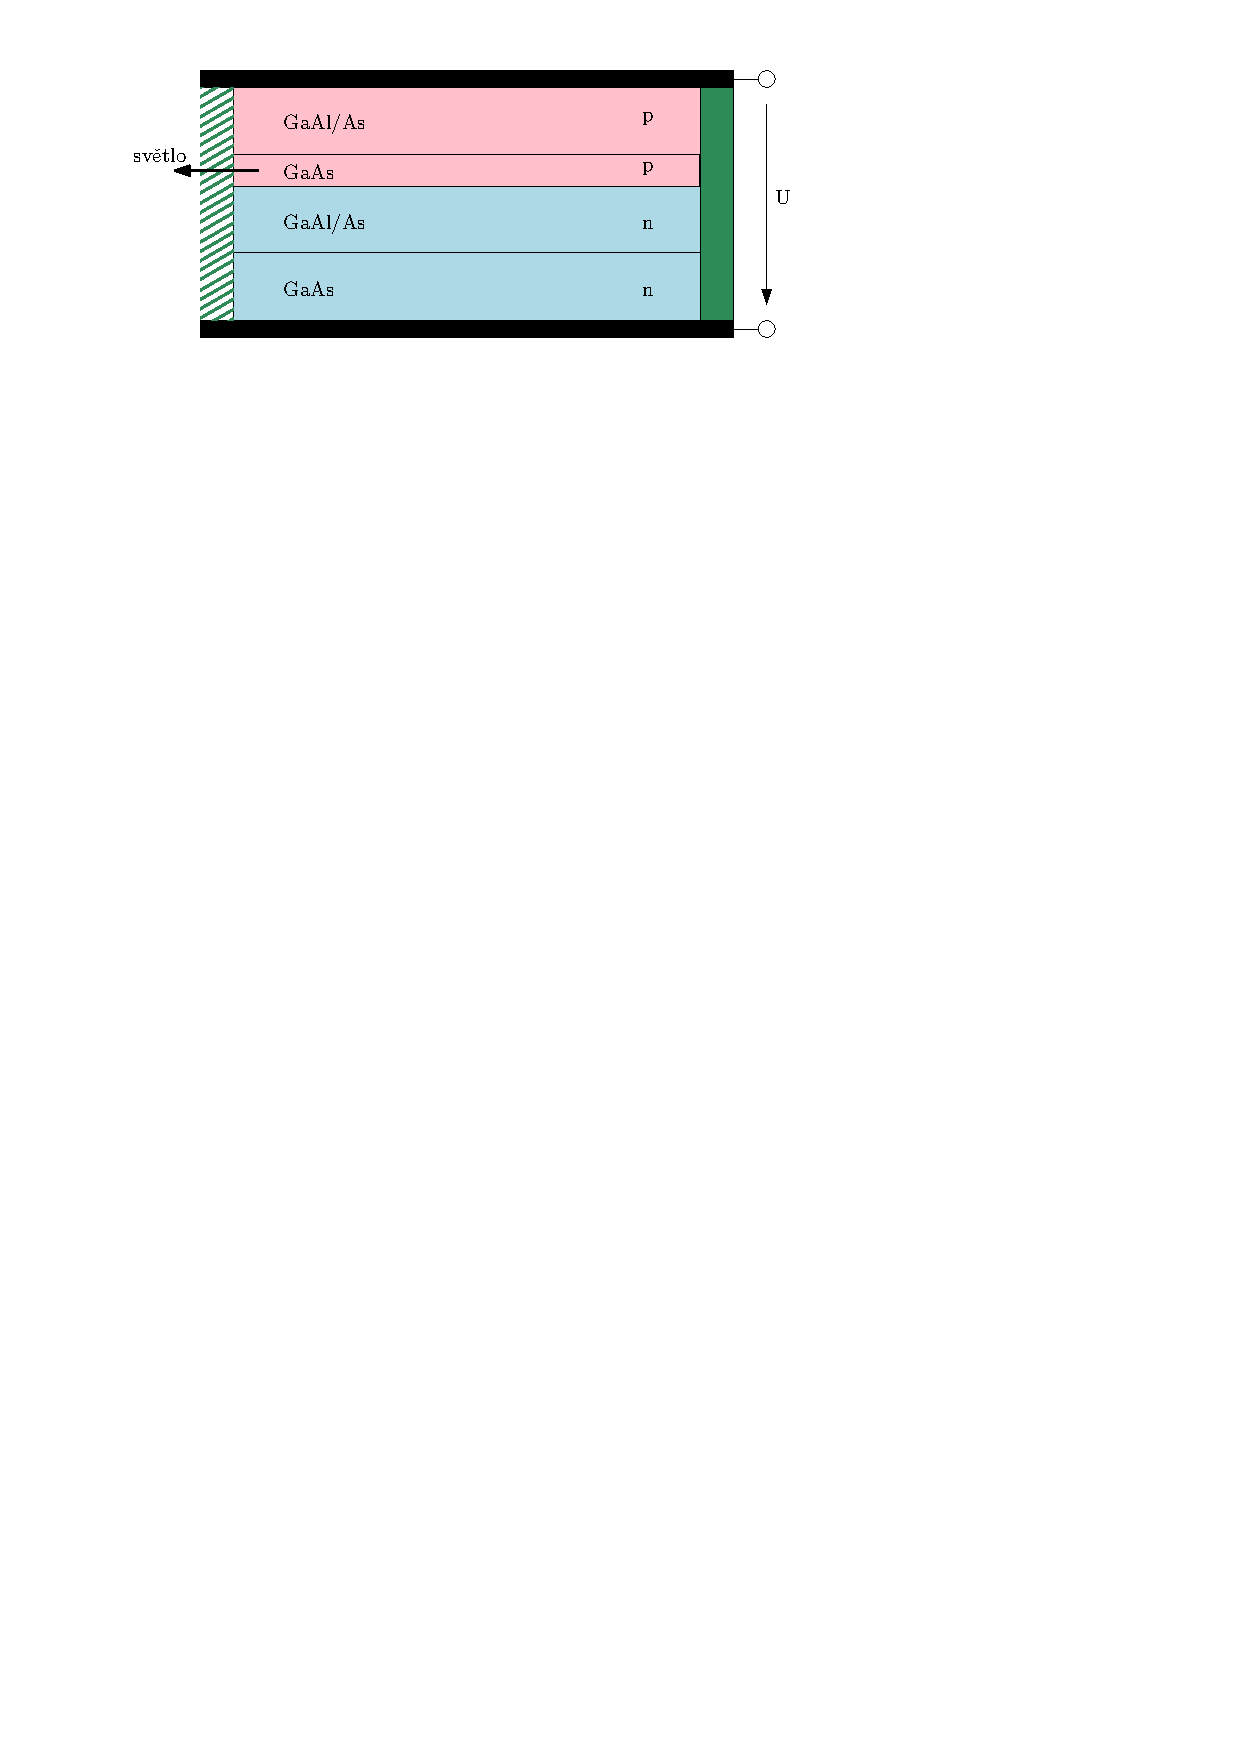
\includegraphics[scale=1]{img/laser}
    \end{center}
    \caption{Dvojitá heterogenní struktura polovodičového laseru}
\end{figure}

Emitované fotony se odráží od zrcadla a polopropustného zrcadla.  Krystal se chová jako dutinový rezonátor. Šířka a výška přechodu udává vid vznikajícího stojatého vlnění. Když překročí intenzita vlnění určitou mez, je vyzářena skrz polopropustné zrcadlo do okolí.

Laserové diody nalézají uplatnění tam, kde je třeba vyzářit velký optický výkon. Vzhledem k tomu, že v laserovém režimu se diody nachází až od vyššího proudu, tak vyžadují dobré chlazení, aby nedošlo k jejich poškození.

\section{Optické přijímače}
Optický přijímač nebo-li detektor či čidlo je elektrotechnická součástka, která převádí elektromagnetické vlnění o vlnových délkách $\lambda \in \langle 1~\jedn{\mu m};~100~\jedn{nm} \rangle$ na elektrickou veličinu, nejčastěji napětí nebo proud.

\subsection{Foto-dioda}
Foto-dioda je polovodičová součástka, založená na fotoelektrickém jevu, která je navržená pro detekování záření. Převádí dopadající elektromagnetické vlny na elektrický proud. Konstrukčně se podobá \zkratka{LED}. Foto-diody se
mohou rozdělit na dvě skupiny a to na PN foto-diody a PIN foto-diody.

Dopadne-li na oblast PN přechodu foton s dostatečnou energii, uvolní z depletiční oblasti jeden pár díra-elektron. Pokud není k diodě přiloženo vnější napětí, je v depletiční oblasti difuzní napětí. Díky difuznímu napětí je elektron urychlen do oblasti N a díra do oblasti P, tím vzniká driftový proud (proud v závěrném směru).

Pokud dopadne foton mimo vyprázdněnou oblast PN přechodu, udělí elektronu energii, díky které se elektron uvolní z valenční vrstvy a stane se volným nosičem náboje. Teprve poté co se elektron dostane do depletiční oblasti, může být urychlen difuzním napětím a tím vznikne difuzní proud. Tento děj je mnohem pomalejší, než pokud foton dopadne přímo do depletiční oblasti.

PN diody nemají moc velkou oblast prostorového náboje, většina záření dopadá mimo oblast prostorového náboje. A elektronům trvá déle, než se dostanou do oblasti prostorového náboje, který je urychlí, aby vytvořili elektrický proud. Díky tomu nejsou vhodné pro detekci rychlých signálů, ale jejich výhodou je díky jejich nízké citlivosti nízká šumovost.

PIN diody jsou oproti PN diodám mnohem rychlejší, mají velkou oblast prostorového náboje a téměř všechny dopadající fotony s dostatečnou energií, uvolní elektron, který je urychlen difuzním napětím a vytvoří záporný driftový proud. Od PN diod se liší tím, že mezi vrstvou N a P mají vrstvu čistého polovodiče s vlastní vodivostí označovanou jako I. Tato vrstva se neuplatňuje při průchodu stejnosměrného proudu, dioda se chová jako běžná PN dioda. Při vyšších frekvencích nosiče náboje z vrstvy I nestihnou být odsáty. Díky tomu má vrstva I lineární odpor daný protékajícím stejnosměrným proudem.

\begin{figure}[H]
    \begin{center}
        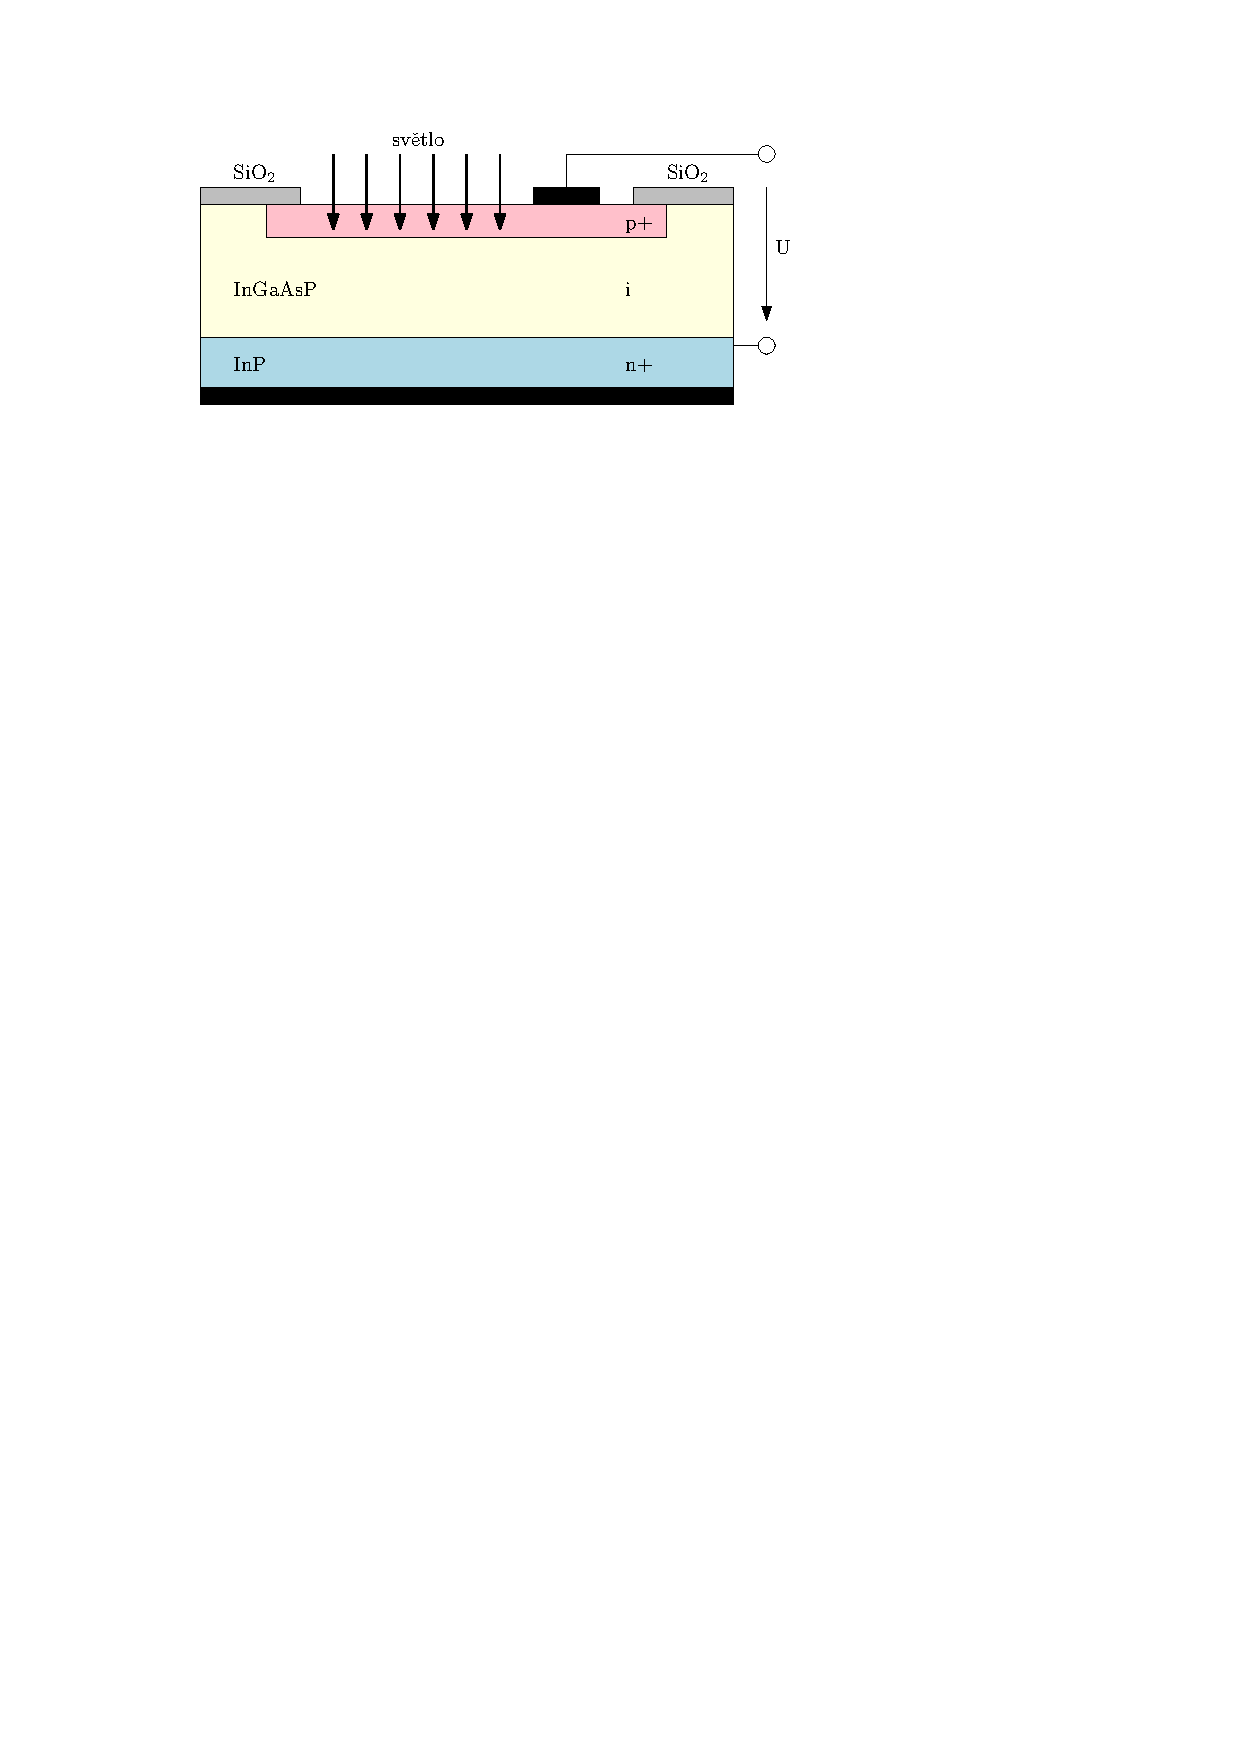
\includegraphics[scale=1]{img/pin}
    \end{center}
    \caption{Struktura PIN diody}
\end{figure}

\subsection{Foto-tranzistor}
Foto-tranzistor se může modelovat jako foto-dioda s tranzistorem jako zesilovačem fotonového proudu. Díky zesílení signálu je schopen detekovat i nižší intenzitu záření. Jeho nevýhodou je, že má $\beta$ větší parazitní kapacitu ($\beta$ je proudový zesilovací činitel), která omezuje jeho mezní frekvenci. Proto není vhodný pro měření rychlých signálů.

\begin{figure}[H]
    \begin{center}
        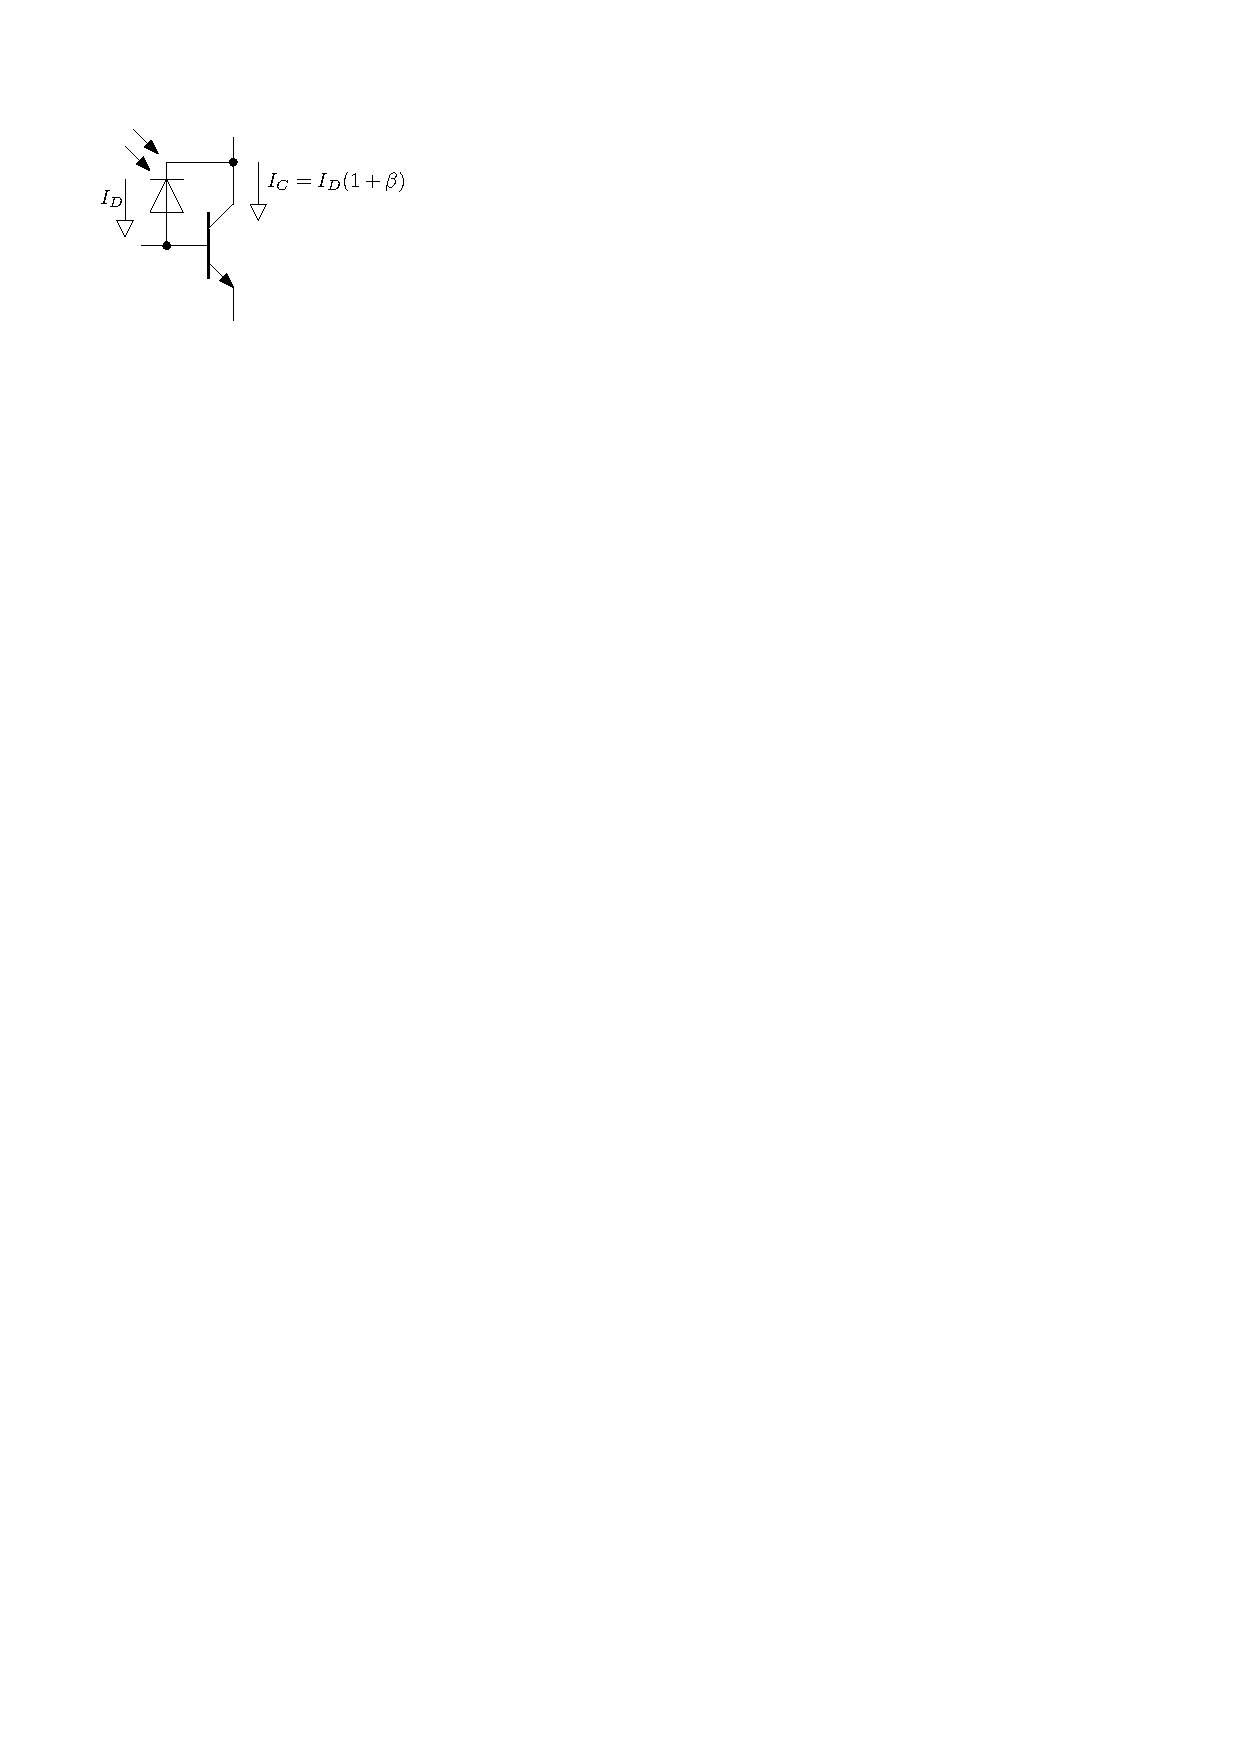
\includegraphics[scale=1]{img/foto-tran}
    \end{center}
    \caption{Náhradní schéma foto-tranzistoru}
\end{figure}

U reálného foto-tranzistoru, dopadají fotony přímo do oblasti báze, není tedy realizovaný foto-diodou s klasickým tranzistorem.

\subsection{Integrované přijímače}
Integrované optické přijímače mají na jednom čipu integrovanou, kromě foto-diody, i další elektroniku. Zpravidla obsahují vstupní zesilovač, pásmovou propust, demodulátor a výstupní zesilovač.

\begin{figure}[H]
    \begin{center}
        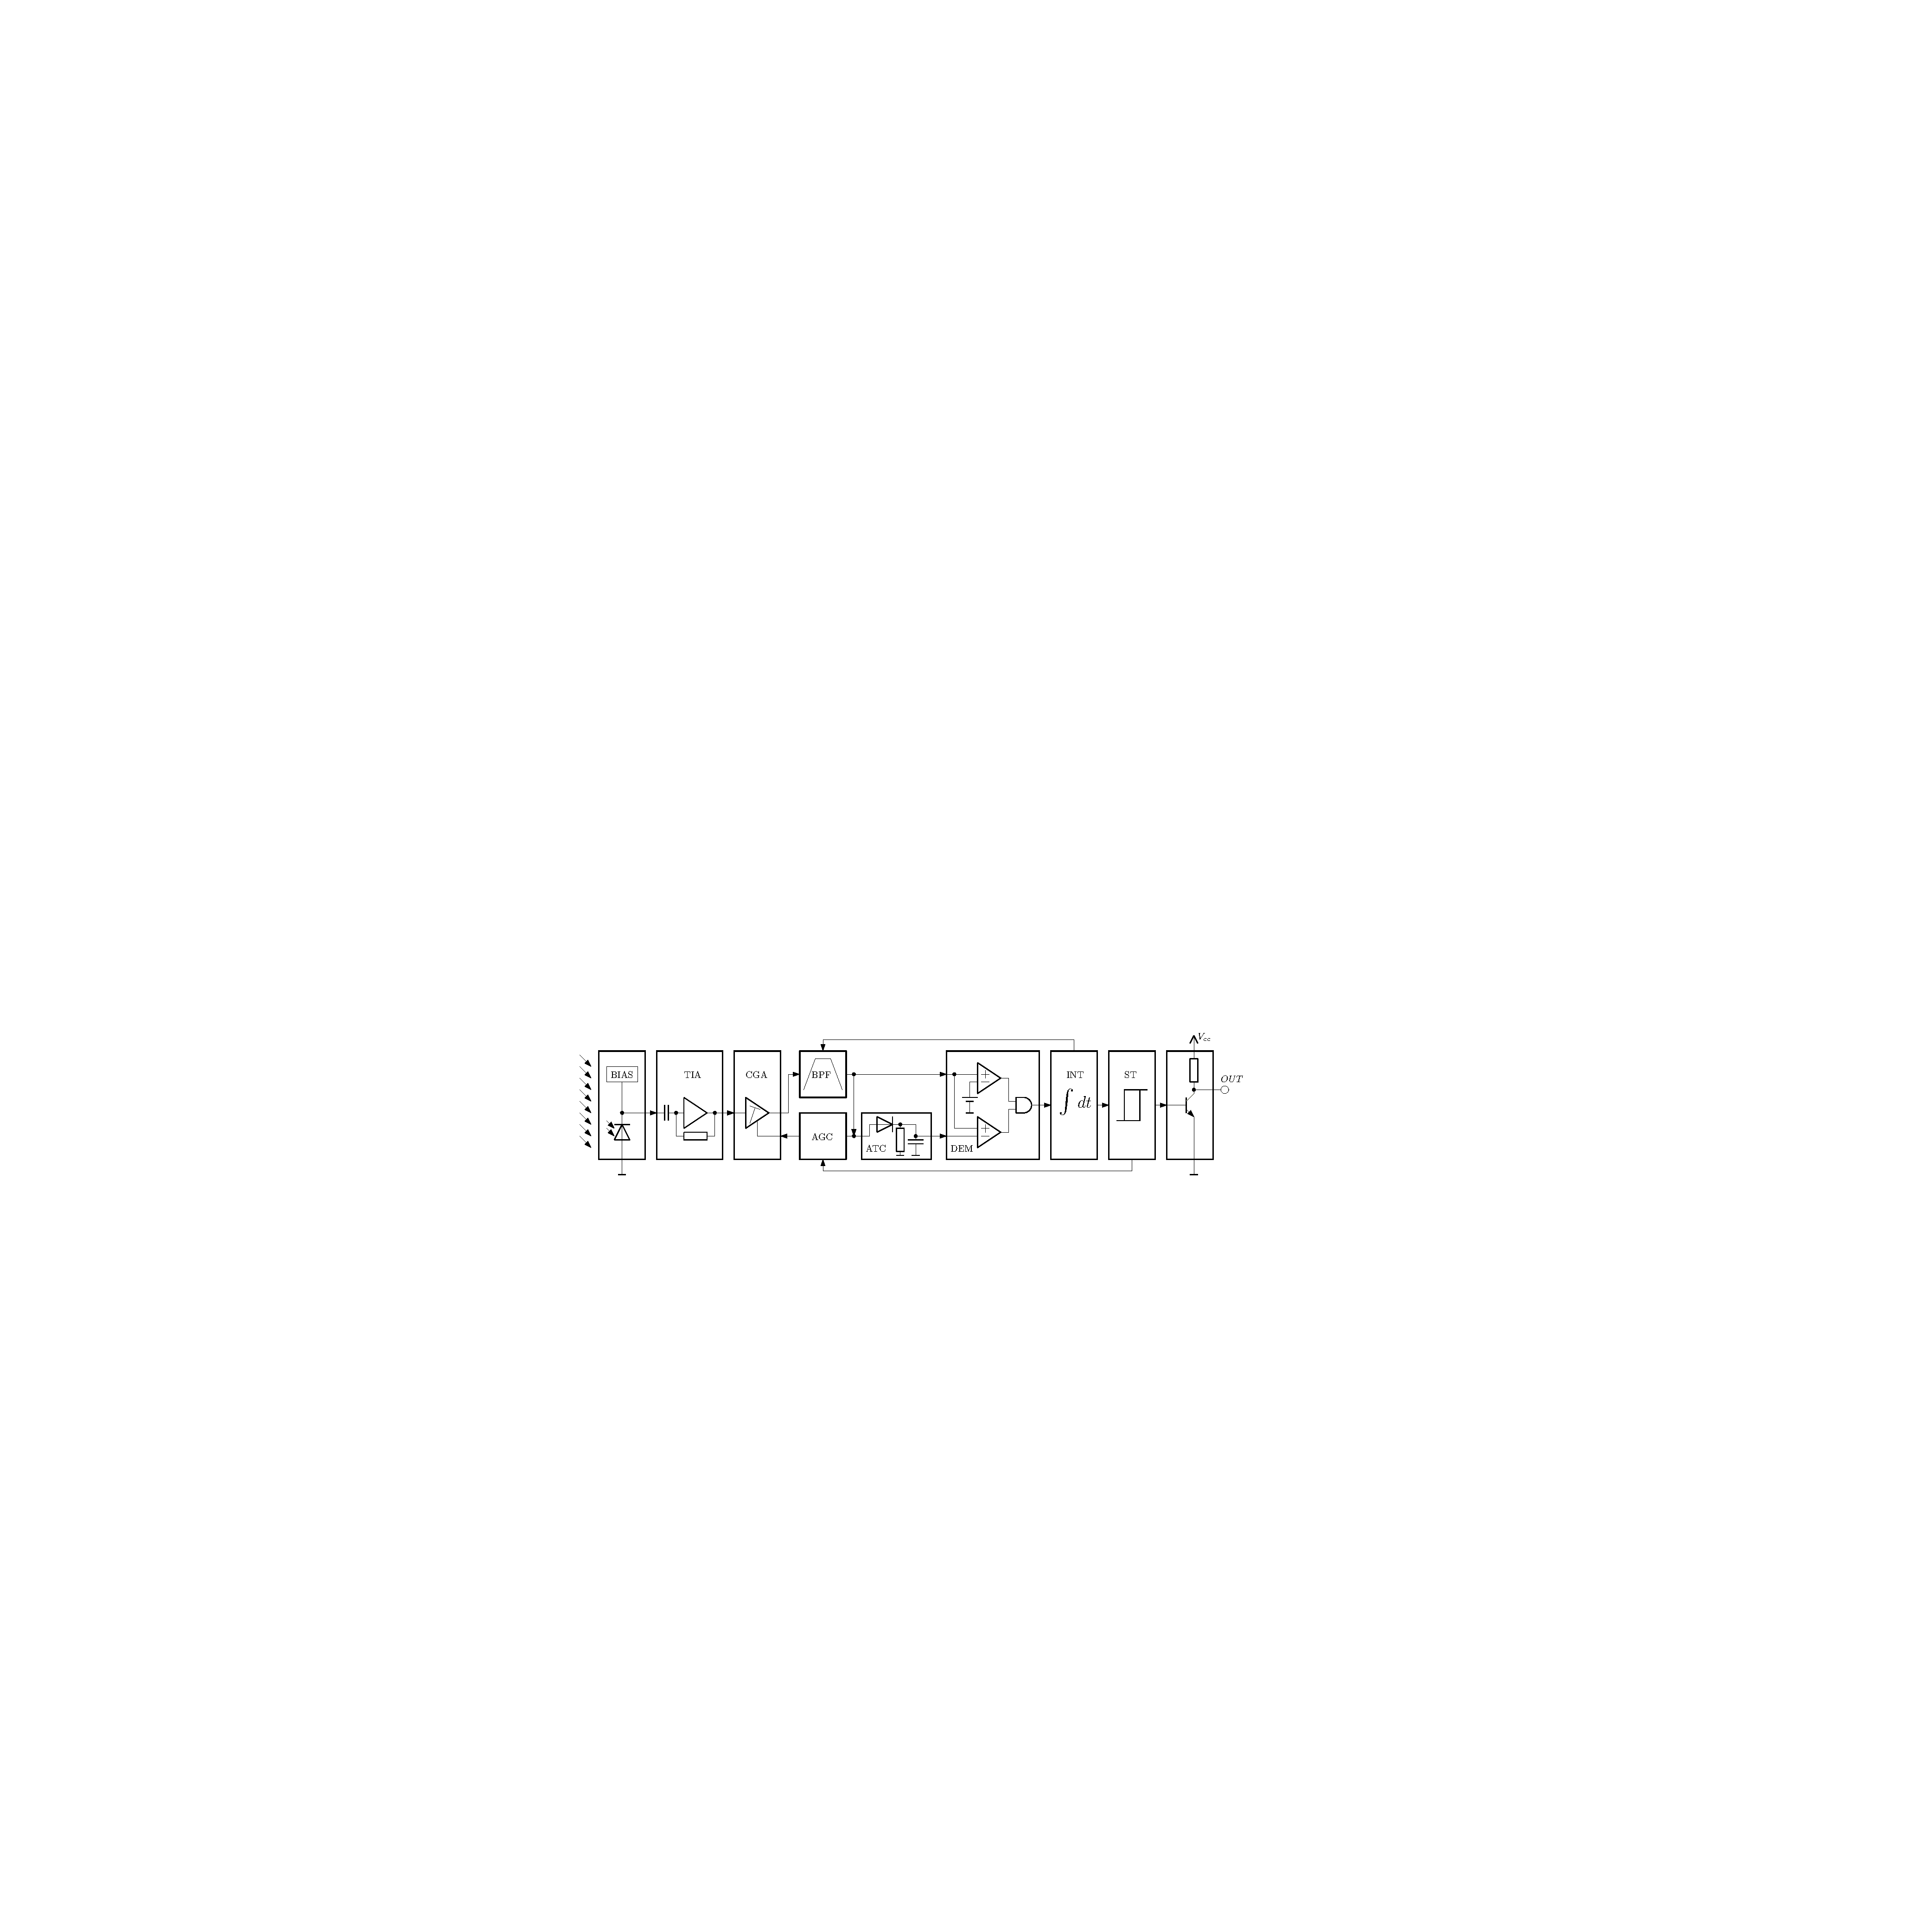
\includegraphics[width=\textwidth]{img/ir-rx}
    \end{center}
    \caption{Blokové schéma integrovaného přijímače OSRB38C9BA}
\end{figure}

Pro konkrétnější popis bude popsán výše uvedený přijímač. Záření v okolí vlnové délky $940~\jedn{\mikro m}$ je detekováno foto-diodou a pomocí trans-impedančního zesilovače (TIA) přivedeno do přijímače. TIA funguje jako napěťový sledovač, který má velký vstupní odpor a malý výstupní odpor. Je tu proto, aby se odebíraným výkonem nezatěžovala foto-dioda.

S TIA je signál přiváděn do zesilovače s nastavitelným zesílením (CGA). Po zesílení je z CGA přiveden na pásmovou propust (BPF) se středním kmitočtem $37,9~\jedn{kHz}$. Ta slouží k odfiltrování rušivých frekvenčních složek před demodulací, aby nevznikali parazitní intermodulační produkty.

Po vyfiltrování se signál rozdělí do dvou větví. První větev jde přímo do demodulátoru. Druhá větev slouží jako jedna ze zpětných vazeb pro CGA. Kromě toho, že druhá větev tvoří zpětnou vazbu vede i do automatického nastavování prahového napětí (ACT), pro druhý komparátor v demodulátoru. Pokud má signál dostatečnou amplitudu, projde diodou a nabije kondenzátor.

Demodulace probíhá tak, že pokud signál, který vychází s BPF má vyšší amplitudu, než je komparační napětí některého z komparátorů, tak komparátor sepne. Aby byl výstup demodulátoru v logické jedničce, tak musí být sepnuté oba dva komparátory, protože jejich výstupy jsou na hradlo AND, které je výstupem demodulace. Tedy vstupní signál musí mít větší amplitudu, než je pevně dané předpětí prvního komparátoru a větší amplitudu než je komparační napětí druhého komparátoru, které je nastavováno z výstupu BPF.

Integrátor vyhlazuje výstupní signál, za cenu toho, že signál ztratí ostré hrany.

Výstup integrátoru je přiveden na vstup Schmittova klopného obvodu, který z integrovaného signálu vytvoří opět ostrý obdélníkový signál. Výstup ze Schmittova komparátoru je další zpětnou vazbu pro CGA a také řídí výstupní tranzistor.
